\documentclass[11pt,a4paper]{article}
\input{~/Documents/latex-config/math-preamble}
\title{DA4005 - Programming Exercise 2}
\author{David Sermoneta}
\date{\today}
\usepackage{epstopdf}
\usepackage{tikz}
\usetikzlibrary{arrows, positioning, calc}
\newcommand{\col}{\genfrac{[}{]}{0pt}{}}
\begin{document}
\maketitle
\section*{Boards and Tiles}
\subsection*{Task 1}
\textbf{(a)} For the first subtask, we want to find the number of ways to cover a cell in
the rightmost column. To do this, notice that a domino can be placed vertically
or horizontally, a monomino can be placed in a unique way, and an L-tromino can
be placed in four ways by taking into account rotations, but one of them will
leave our cell uncovered, so the number of contributions is three. Putting
these together, we get that there are in total $1 + 2 + 3 = 6$ ways to cover a
cell in the rightmost column. This is obviously not taking into account if the cell under/above the cell we want to cover is already covered or not. If that is the case then there is a case-analysis to be made.

\noindent \textbf{(b)} Our program works in the following way: We construct all
possible tilings of a $2\times k$ board for all $k \leq n$, using the previous
constructions to create the next. We represent the board with the help of lists
of lists of 2 elements, or list of columns, ordered in the obvious way. We
start off with a list of one column, and create all possible tilings of it,
namely two monominoes, or a vertical domino. Here is a good place to talk about
how the different tiles are represented. Tiling a board is achieved by filling
up a list of columns, and an example might be the best way to showcase how (and
hopefully why) we have chosen to represent the filled cells. For the board given
in the description, our program would write it as \[
\texttt{[ [7,7], [7,1], [2,2], [2,2], [7,7], [7,1], [3,3] ]},
\] i.e., representing the ($2\times 7$) board 
\begin{center}
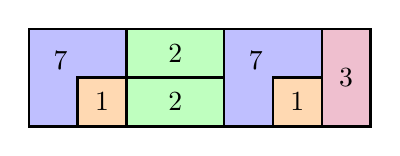
\begin{tikzpicture}[x=0.62cm,y=0.62cm,thick]
  \draw[fill=blue!25]
    (0,0)--(1,0)--(1,1)--(2,1)--(2,2)--(0,2)--cycle;
  \node at (0.65,1.35) {$7$};
  \draw[fill=orange!30] (1,0) rectangle (2,1);
  \node at (1.5,0.5) {$1$};
  \draw[fill=green!25] (2,0) rectangle (4,1);
  \node at (3,0.5) {$2$};
  \draw[fill=green!25] (2,1) rectangle (4,2);
  \node at (3,1.5) {$2$};
  \draw[fill=blue!25]
    (4,0)--(5,0)--(5,1)--(6,1)--(6,2)--(4,2)--cycle;
  \node at (4.65,1.35) {$7$};
  \draw[fill=orange!30] (5,0) rectangle (6,1);
  \node at (5.5,0.5) {$1$};
  \draw[fill=purple!25] (6,0) rectangle (7,2);
  \node at (6.5,1) {$3$};
\end{tikzpicture}
\end{center}
The choice of numbering is just convenient notation to be able to distinguish between the different rotations of the tiles. This also has the convenient benefit of only requiring us to check the last column when wanting to compute all the $2\times n$ extensions of a $2\times (n-1)$ board. The notation is further explained in the documentation for the class $\texttt{Board}$ in the code.

Since we mentioned extending boards, it makes sense to talk about that next. We
have indeed a function $\texttt{extend(lastCol)}$ which is
supposed to take in the last column from a board, and then output all possible
$2\times 2$ boards that can be made from that column, given the restriction of
how the tiles can be arranged in the last column, and which tiles are allowed.
 Then we generate new boards by stitching together the old board with all the new $2\times 2$ boards.
By how we have implemented our representation, this has $9$ cases to check,
because there are only $9$ ways the last column can look, these are given by
\[
\col{2}{2}, \col{4}{4}, \col{6}{6}, \col{2}{1}, \col{1}{2},  \col{3}{3}, \col{1}{5}, \col{7}{1}, \col{1}{1}.
\] 
The first three cases only have $2$ possible extensions, since they cannot be
transformed without creating an unvalid tiling, and so we are only adding an
already filled column, there are $2$ ways to do this. From the fourth to the
next-to-last column, there are $4$ extensions, two given by the same argument
as in the previous three, and two by the only allowed transformations that end
up in a completely new tiling, as given by our example below. The last case,
with a monomino in each cell, can naturally be extended into the most amount of
new tilings, which is $7$. Two of these are again, because we can just extend
trivially. Three are given by all the ways we can turn one or two monominoes
into parts of horizontal dominoes. Finally, the last two extensions are given by the
 ways we can turn one monomino into an L-tromino. The reason we exclude say,
turning both monominoes into a vertical domino is because that would turn into
the same cases as the one with a vertical domino already! 

We illustrate this by running $\texttt{extend}$ on the last column of our previous example, the $2\times 7$ is extendable into $4$ new $2\times 8$ boards,
 since we can either leave the rightmost vertical domino as it is, giving us
two extensions (by a vertical domino or two monominoes), but it is also a valid
extension to turn the domino into an L-trominoes, and then extend with the rest
of the L-tromino and supplementary monomino either below or above it (giving us
two more extensions). 
\begin{center}
% Extension 1: add a vertical domino
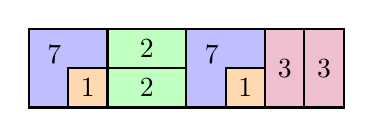
\begin{tikzpicture}[x=0.5cm,y=0.5cm,thick]
  \draw[fill=blue!25]
    (0,0)--(1,0)--(1,1)--(2,1)--(2,2)--(0,2)--cycle;
  \node at (0.65,1.35) {$7$};
  \draw[fill=orange!30] (1,0) rectangle (2,1);
  \node at (1.5,0.5) {$1$};
  \draw[fill=green!25] (2,0) rectangle (4,1);
  \node at (3,0.5) {$2$};
  \draw[fill=green!25] (2,1) rectangle (4,2);
  \node at (3,1.5) {$2$};
  \draw[fill=blue!25]
    (4,0)--(5,0)--(5,1)--(6,1)--(6,2)--(4,2)--cycle;
  \node at (4.65,1.35) {$7$};
  \draw[fill=orange!30] (5,0) rectangle (6,1);
  \node at (5.5,0.5) {$1$};
  \draw[fill=purple!25] (6,0) rectangle (7,2);
  \node at (6.5,1) {$3$};

  % New vertical domino
  \draw[fill=purple!25] (7,0) rectangle (8,2);
  \node at (7.5,1) {$3$};
\end{tikzpicture}
\hspace{1cm}
% Extension 2: two monominoes
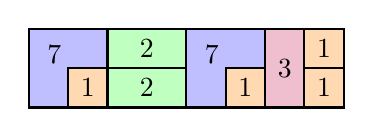
\begin{tikzpicture}[x=0.5cm,y=0.5cm,thick]
  \draw[fill=blue!25]
    (0,0)--(1,0)--(1,1)--(2,1)--(2,2)--(0,2)--cycle;
  \node at (0.65,1.35) {$7$};
  \draw[fill=orange!30] (1,0) rectangle (2,1);
  \node at (1.5,0.5) {$1$};
  \draw[fill=green!25] (2,0) rectangle (4,1);
  \node at (3,0.5) {$2$};
  \draw[fill=green!25] (2,1) rectangle (4,2);
  \node at (3,1.5) {$2$};
  \draw[fill=blue!25]
    (4,0)--(5,0)--(5,1)--(6,1)--(6,2)--(4,2)--cycle;
  \node at (4.65,1.35) {$7$};
  \draw[fill=orange!30] (5,0) rectangle (6,1);
  \node at (5.5,0.5) {$1$};
  \draw[fill=purple!25] (6,0) rectangle (7,2);
  \node at (6.5,1) {$3$};

  % Two new monominoes
  \draw[fill=orange!30] (7,0) rectangle (8,1);
  \node at (7.5,0.5) {$1$};
  \draw[fill=orange!30] (7,1) rectangle (8,2);
  \node at (7.5,1.5) {$1$};
\end{tikzpicture}

\vspace{1cm}

% Extension 3: L-tromino 7 + monomino
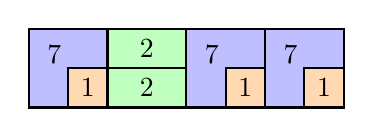
\begin{tikzpicture}[x=0.5cm,y=0.5cm,thick]
  \draw[fill=blue!25]
    (0,0)--(1,0)--(1,1)--(2,1)--(2,2)--(0,2)--cycle;
  \node at (0.65,1.35) {$7$};
  \draw[fill=orange!30] (1,0) rectangle (2,1);
  \node at (1.5,0.5) {$1$};
  \draw[fill=green!25] (2,0) rectangle (4,1);
  \node at (3,0.5) {$2$};
  \draw[fill=green!25] (2,1) rectangle (4,2);
  \node at (3,1.5) {$2$};
  \draw[fill=blue!25]
    (4,0)--(5,0)--(5,1)--(6,1)--(6,2)--(4,2)--cycle;
  \node at (4.65,1.35) {$7$};
  \draw[fill=orange!30] (5,0) rectangle (6,1);
  \node at (5.5,0.5) {$1$};

  % L-tromino: old domino + lower cell of new column
  \draw[fill=blue!25]
    (6,0)--(7,0)--(7,1)--(8,1)--(8,2)--(6,2)--cycle;
  \node at (6.65,1.35) {$7$};

  % Monomino in remaining cell
  \draw[fill=orange!30] (7,0) rectangle (8,1);
  \node at (7.5,0.5) {$1$};
\end{tikzpicture}
\hspace{1cm}
% Extension 4: flipped L-tromino 5 + monomino
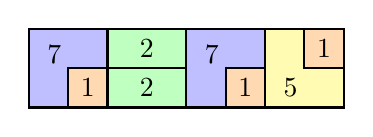
\begin{tikzpicture}[x=0.5cm,y=0.5cm,thick]
  \draw[fill=blue!25]
    (0,0)--(1,0)--(1,1)--(2,1)--(2,2)--(0,2)--cycle;
  \node at (0.65,1.35) {$7$};
  \draw[fill=orange!30] (1,0) rectangle (2,1);
  \node at (1.5,0.5) {$1$};
  \draw[fill=green!25] (2,0) rectangle (4,1);
  \node at (3,0.5) {$2$};
  \draw[fill=green!25] (2,1) rectangle (4,2);
  \node at (3,1.5) {$2$};
  \draw[fill=blue!25]
    (4,0)--(5,0)--(5,1)--(6,1)--(6,2)--(4,2)--cycle;
  \node at (4.65,1.35) {$7$};
  \draw[fill=orange!30] (5,0) rectangle (6,1);
  \node at (5.5,0.5) {$1$};

  % Flipped L-tromino: old domino + upper cell of new column
  \draw[fill=yellow!30]
    (6,0)--(8,0)--(8,1)--(7,1)--(7,2)--(6,2)--cycle;
  \node at (6.65,0.5) {$5$};

  % Monomino in remaining cell
  \draw[fill=orange!30] (7,1) rectangle (8,2);
  \node at (7.5,1.5) {$1$};
\end{tikzpicture}
\end{center}

The ``recursion'' happens essentially in the $\texttt{extend}$ function. This
is because each computation of the possible $2\times n$ tilings is based on all
the $2\times (n-1)$ tilings. Since we create an entirely new tiling and don't
remove the earlier ones, this takes copious amounts of memory resources, so for
computing actual cardinalities of tilings, we make use of a recurrence formula
that bypasses actually tiling a board, and instead just computes the number
based on a little combinatorics, similar to what we did for the
$\texttt{extend}$ function. Here symmetry is exploited more, and the
documentation argue sufficiently why that is enough.

I did decide to write the program saving each set of $2\times k$ tilings in a dictionary for my own purposes which maybe technically disqualifies it from being a 
dynamic program, but one could easily amend this by just having two list variables,
and calling $\texttt{extend}$ on the first list, storing the results in the second, and then call the function again on the second list and store the values in the first and so on until we have done this $n$ times.

\textbf{(c)} If $T(n)$ is the number of tilings of a $2\times n$ board. By convention, we set $T(0) = 1$, since the empty tiling is \textit{obviously} a tiling. Then 
we have that  \[
 T(1) = 2, T(2) = 11 \text{ and } T(3) = 44.
\] 

\subsection*{Task 2}
\textbf{(a)} The number of complete tilings is given by $T(10) = 1089155$.
\textbf{(b)} Minimizing the number of tilings just means maximising the number of L-trominoes. Let $n$ be the number of columns. Then there are three cases to consider:
if  $n \equiv_{3} 0$, then an optimal tiling is given by repeated L-trominos in an interlocking fashion. 
If $n\equiv_{3} 1$, we do the same, but the last column gets filled by a vertical domino, and if $n \equiv_{3} 2$, we just add another L-tromino, in any orientation, and then insert a monomino (or equivalently, two dominoes). 

\textbf{(c)} One estimate for the upper bound of the runtime is to just assume
all previous tilings always end in a double monomino configuration, since that is the case with the most branching. For each of those, we get that
the runtime is $7^{n}$. For a lower bound, we get $2^{n}$, which is still exponential.
Obviously the actual runtime lies somewhere in between, since there are obviously more cases to check than just these two. If we instead look at the runtime of our recursion counting formula, we have that it's linear in $n$, since we are just making a few coputations, storing them, and then updating a value $n$ times in total.

\subsection*{Task 3}
We begin by proving \textbf{(*)}, as that will get me most bragging rights, as well as making our dynamic program simpler to implement.

Let $$
B_1(n) = \left|\{2\times n \text{ tilings ending with two
monominoes}\}\right|.
$$
Similarly,
\begin{align*}
B_2(n) =& \{\text{tilings ending with a vertical domino}\} \\
B_3(n) = & \frac{1}{2} \left|\{\text{tilings ending with a horizontal domino and monomino}\}\right| = B_4(n) \\
B_5(n) = & \frac{q}{2} \left| \{ \text{tilings whose last column is filled by a single L-tromino} \}\right| = B_6(n)\\
B_7(n) =& \frac{q}{2}\left|\{ \text{tilings whole last column is an L-tromino and a monomino}\}\right| \\
 B_9(n) = & \left|\{\text{tilings ending with two horizontal dominoes.}\}\right| \\
\end{align*}
Here we have matched together ending tilings that are just a
 reflection of eachother, and added a factor of $q$ for $B_7$ and
 $B_5$, since all the tilings contributing to this amount also contribute an extra L-tromino to the mix. Furthermore, we have that \[
 P_{n}(q) = \sum_{k=1}^{9} B_{k}(n) = B_1(n) + B_2(n) + 2B_3(n) + 2B_6(n) + 2B_7(n) + B_9(n).
 \]
Furthermore, the shape of the last two columns of the tilings contributing to the total of $B_3$ and $B_4$ are the same as those contributing to the total of $B_5$ and $B_6$, and the same is true for $B_1$ and $B_2$ and $B_7, B_8$ and $B_9$. Therefore, 
the above can be simplified further into \[
P_{n}(q) = 2B_1(n) + (2 + 2q)B_3(n) + (1 + 2q)B_9(n).
\] 
Now by the same reasoning as in the lecture notes, $B_1(n) = P_{n-1}(q)$, and 
$B_9(n) = P_{n-2}(q)$.  Therefore, we end up with a yet more simplified version of $P_{n}(q)$ namely \[
P_{n}(q) = 2P_{n-1}(q) + (2+ 2q)B_3(n) + (1+2q) B_9(n).
\] 
Now we would like to rewrite that $B_3(n)$ term in terms of our polynomial, 
but we only have that \[
B_3(n) = B_1(n-1) + B_3(n-1) + B_7(n-1),
\] because if we remove the last column of a tiling ending in a monomino and horizontal domino, we can tile the last column of this $2\times (n-1)$ tiling only in ways that ends us up with one of the three tilings represented above (modulo a $\Z /2\Z$ -action on the space of tilings). The above also gives us the relation  
\[
B_3(n) - B_3(n-1) = B_1(n-1) + B_7(n-1) = P_{n-2}(q) + qP_{n-3}(q),
\] and we can get this to work by subtracting $P_{n-1}(q)$ from 
$P_{n}(q)$. Then we get 
\begin{align*}
P_{n}(q) - P_{n-1}(q) = & 2(P_{n-1}(q) - P_{n-2}(q)) + (2+2q)(B_3(n) - B_3(n-1)) + \\
 +& (1+2q)(P_{n-1}(q) - P_{n-2}(q)) \\
=& 2(P_{n-1}(q) - P_{n-2}(q)) + (2+2q)(P_{n-2}(q) + qP_{n-3}(q)) + \\
+& (1+2q)(P_{n-2}(q) - P_{n-3}(q)).
\end{align*}
Simplifying this further we finally get that \[
P_{n}(q) = 3P_{n-1}(q) + (4q +1)P_{n-2}(q) + (2q^2 - 1)P_{n-3}(q),
\] and so we are done.
\noindent \textbf{(a) and (b)} Now we can implement this recursion formula to get a dynamic program that returns $P_{n}(q).$ This is given by the function \newline 
$\texttt{computePolyDynamically(n)}$ making use of the symbolic package $\texttt{sympy}$.
\end{document}
